\chapter{Entwicklung der Methodik}
\label{ch:EntwicklungDerMethodik}
Die in Kapitel \ref{ch:StandTechnik} vorgestellten Ansätze bilden die theoretische Grundlage dieser Arbeit. Um ein robustes Feature-Extraktionssystem zu entwickeln, ist jedoch eine Anpassung und Weiterentwicklung bestehender Methoden erforderlich. Dieses Kapitel beschreibt den iterativen Prozess, der zur finalen Konzeption und Architektur führt. Es beleuchtet die anfängliche Analyse des zugrundeliegenden Papers von \textcite{He_2023_ICCV}, die identifizierten Herausforderungen sowie die Lösungsansätze, die zur Überwindung dieser Probleme entwickelt werden. Die hier getroffenen Entscheidungen bilden die konzeptionelle Brücke zwischen dem Stand der Technik und der eigentlichen Implementierung.





\section{Analyse des He-Papers und Ausgangslage}
\label{sec:Analyse}
Die Grundlage für die Entwicklung der Methodik ist die Forschungsarbeit von \textcite{He_2023_ICCV} zum Thema Shape-Bias. Der zentrale Gedanke dieser Arbeit ist die Annahme, dass der Mensch Objekte primär anhand ihrer Form (Shape) erkennt, während neuronale Netze oftmals auf Texturmerkmale (Texture) trainiert werden. Dieses Verhalten, der sogenannte Texture-Bias, kann insbesondere in Umgebungen mit variablen Lichtverhältnissen oder sich ändernden Oberflächen zu fehlerhaften Schlussfolgerungen führen. Um die Erkennung auf die Form des Objekts zu fokussieren, schlagen \textcite{He_2023_ICCV} einen Ansatz zur Daten-Augmentierung vor, der die Textur eines Bildes reduziert, während die Kanten und die semantische Form des Objekts verstärkt werden.

\subsection{Architektur des Generative Adversarial Networks (GANs)}
Das Herzstück der Methode von \textcite{He_2023_ICCV} ist ein \ac{GAN}, das in der Lage ist, Bilder so zu modifizieren, dass sie eine reduzierte Textur aufweisen und Kanten verstärkt werden. Die Architektur besteht aus einem Generator- und einem Diskriminator-Netzwerk, die in einem Minimax-Spiel gegeneinander trainiert werden (siehe Abbildung~\ref{fig:GAN_Aufbau}). Der Generator ($G$) lernt, aus einem Originalbild ($I_{orig}$) und einer zugehörigen Kantenkarte ($E$) ein synthetisches Bild ($I_{syn}$) zu erzeugen. Der Diskriminator ($D$) lernt, zwischen echten und synthetischen Bildern zu unterscheiden. Dieses kompetitive Training zwingt den Generator, Bilder zu erzeugen, die für den Diskriminator nicht von der Realität zu unterscheiden sind. Die Kantenkarte wird über den gesamten Prozess als eine Art \enquote{Shape-Guidance} verwendet, die den Generator dazu anleitet, die Form des ursprünglichen Objekts zu bewahren.

\begin{figure}[htpb]
    \centering
    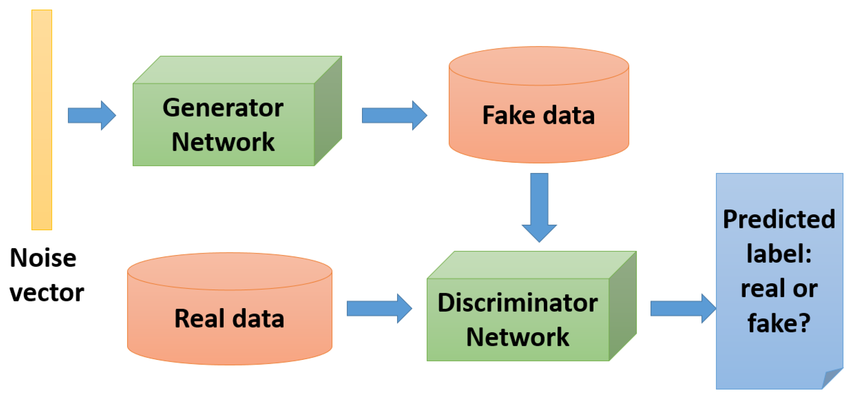
\includegraphics[clip, trim=0cm 0cm 0cm 0cm, width=\VarPicWidthD]{Figures/png/GAN_Aufbau.png}
    \caption{Schematische Darstellung der GAN-Architektur nach \textcite{Benjdira2019GAN}}
    \label{fig:GAN_Aufbau}
\end{figure}

\newpage




\subsection{Zweistufiger Trainingsprozess}
Das Modell wird in einem zweistufigen Prozess trainiert:

\begin{itemize}
    \item \textbf{Stage 1: Generierung textur-reduzierter Bilder.} In der ersten Phase wird der Generator auf einem Datensatz wie CIFAR-10~\cite{krizhevsky2009learning} oder ImageNet256~\cite{Uriot2023imageNet} trainiert, um aus einem Originalbild ein neues Bild zu erzeugen, das dieselbe Form und Geometrie, aber eine reduzierte Textur aufweist. Der Fokus liegt hierbei auf der photorealistischen Nachbildung der Form, während die textuellen Details bewusst unterdrückt werden.
    \item \textbf{Stage 2: Fine-Tuning mit Kantenverformung.} In der zweiten Phase wird der Generator mit deformierten Kantenkarten gefüttert, um zu lernen, wie dieser plausible Bilder mit manipulierten Formen erzeugen kann. Laut \textcite{He_2023_ICCV} sollen diese Deformationen einen nachfolgenden Klassifizierer dazu bringen mehr auf die Form eines Objekts zu achten und weniger auf die Textur.
\end{itemize}




\subsection{Anfängliche Umsetzung und Zielsetzung}
Die Ausgangslage für die vorliegende Arbeit ist die Replikation und Adaption dieser Architektur für die spezifischen Anforderungen im Visual Servoing. Der Fokus liegt darauf, die Stärken des Konzepts zu nutzen, um den Shape-Bias im Keypoint-Detektor \textbf{\ac{xFeat}} zu stärken und somit robustere Merkmale zu erhalten. Diese Merkmale sollen in einem nachgelagerten Regelverfahren zur Positionskontrolle genutzt werden, um eine höhere Präzision und Stabilität zu erreichen. Unsere anfängliche Umsetzung orientiert sich daher strikt an den Prinzipien und der vorgeschlagenen Architektur von \textcite{He_2023_ICCV}, um die Funktionalität und die Machbarkeit des Ansatzes zu überprüfen. Im Gegensatz zur Originalarbeit, welche CIFAR-10~\cite{krizhevsky2009learning} mit einer Auflösung von $32 \times 32$ Pixeln verwendet, adaptieren wir das Vorgehen auf den ImageNet256 Datensatz~\cite{Uriot2023imageNet} mit Bildern der Größe $256 \times 256$ Pixeln. Dies ist eine notwendige Anpassung, da der nachfolgende Keypoint-Detektor und Deskriptor \ac{xFeat} mit hochauflösenden Bildern trainiert wird ($800 \times 608$ Pixeln). Die Skalierung des Ansatzes auf größere Bildauflösungen ist somit ein zentrales Element unserer Arbeit und bildet die Grundlage für die hier beschriebenen Weiterentwicklungen.





\section{Herausforderungen und Lösungsansätze}
\label{sec:HerausforderungenUndLoesungsansaetze}
Die direkte Übertragung des Ansatzes von \textcite{He_2023_ICCV} auf den ImageNet256 Datensatz~\cite{Uriot2023imageNet} mit einer höheren Bildauflösung führt zu diversen Herausforderungen. Es stellt sich heraus, dass das ursprüngliche Konzept, insbesondere die Methode zur Kantenextraktion, nicht ohne Weiteres auf die neuen Bedingungen anwendbar ist. Die zentralen Probleme sind die unzureichende Nutzung der Kantenkarte durch den Generator und die limitationsbedingte Ineffizienz des ursprünglichen Kantenextraktionsverfahrens. Außerdem muss das vorliegende Generator-Netz auf die erhöhte Bildgröße, $32 \times 32$ vs. $256 \times 256$ Pixeln, angepasst werden.




\subsection{Herausforderung 1: Ineffektive Nutzung der Kantenkarte}
Bei der anfänglichen Umsetzung stellen wir fest, dass der Generator die zur Verfügung gestellte Kantenkarte, die als Leitfaden für die Form dienen soll, nahezu ignoriert. Stattdessen extrahiert er die notwendigen Forminformationen primär aus dem texturreduzierten Eingangsbild.  Dieses Verhalten, das durch unser Diagnosetool nachgewiesen wird, deutet auf einen weiterhin bestehenden Texture-Bias hin, auch wenn die Textur nur in geringem Maße vorhanden ist. Die Annahme, dass der Generator bei fehlender Textur automatisch auf die Kantenkarte zurückgreift, bewahrheitet sich nicht. Wir identifizieren, dass die Informationen im texturreduzierten Bild auch bei einer Downsampling-Rate von $16 \times 16$ Pixeln noch zu dominant sind und das Netzwerk somit keinen Anreiz hat, die Kantenkarte zu nutzen.




\subsection{Lösungsansatz 1: Einführung einer dynamischen Texturreduktion}
Um den Shape-Bias zu fördern, entwickeln wir eine erweiterte Methode zur Texturreduktion, die den Texture-Bias des Generators gezielt unterdrückt. Unser Lösungsansatz besteht darin, einen variablen Gaussian Blur auf die Eingangsbilder anzuwenden. Dadurch können wir die Intensität der Texturreduktion dynamisch steuern und so einen stärkeren Trainingsreiz auf die Kantenkarte ausüben. Zusätzlich wird eine probabilistische Methode implementiert, die das Eingangsbild mit einer bestimmten Wahrscheinlichkeit vollständig von Texturinformationen befreit (sogenannter Texture-Dropout).

\newpage




\subsection{Herausforderung 2: Inkompatibilität des Kantenextraktionsverfahrens}
Die ursprüngliche Methode zur Kantenextraktion, der sogenannten \ac{EMSE}, die auf dem nicht-differenzierbaren Canny-Algorithmus basiert, ist für eine End-to-End-Trainingspipeline in PyTorch ungeeignet. Die Notwendigkeit, einen \ac{CPU}-Transfer für die Kantenberechnung durchzuführen, unterbricht den Backpropagation-Prozess und führt zu einem erheblichen Leistungsverlust. Um eine nahtlose und effiziente Integration zu ermöglichen, ist ein vollständig differenzierbares und \ac{GPU}-basiertes Verfahren zur Kantenextraktion erforderlich, das direkt in die Verlustfunktion integriert werden kann.

Zudem erweist sich die \ac{EMSE}-Methode als unzureichend für die Extraktion von qualitativ hochwertigen Kantenkarten aus Bildern mit einer Auflösung von $256 \times 256$ Pixeln. Während sie bei den kleineren $32 \times 32$ Pixel-Bildern des CIFAR-10-Datensatzes~\cite{krizhevsky2009learning} noch akzeptable Ergebnisse liefert, verliert sie bei größeren und komplexeren Bildern an Effektivität. Die unzureichende Qualität der Eingangs-Kantenkarten beeinträchtigt die Fähigkeit des Generators, robuste, formbasierte Merkmale zu lernen, da die primäre Quelle für die Forminformationen nicht ausreichend ist.




\subsection{Lösungsansatz: Entwicklung von DS-EMSE}
Als Antwort auf die Inkompatibilität des ursprünglichen Kantenextraktionsverfahrens entwickeln wir die \ac{DS-EMSE} Methode. Diese vollständig differenzierbare Kantenextraktion basiert auf dem Sobel-Filter und ist direkt in die PyTorch-Pipeline integrierbar. Im Gegensatz zum binären Canny-Algorithmus erzeugt unser Verfahren eine Graustufen-Kantenkarte, die die Stärke der Kanten repräsentiert. Dies liefert eine höhere Informationsdichte und ermöglicht eine bessere Nutzung der Kantendaten durch den Generator. Die durchgängige Differenzierbarkeit eliminiert nicht nur den ineffizienten \ac{CPU}-Transfer, sondern verbessert auch die Qualität der Verlustrückpropagierung, was das Training stabilisiert. Der Aufbau der \ac{DS-EMSE} ist in Abbildung \ref{fig:DS_Emse_Ablauf} dargestellt.

\begin{figure}[htpb]
    \centering
    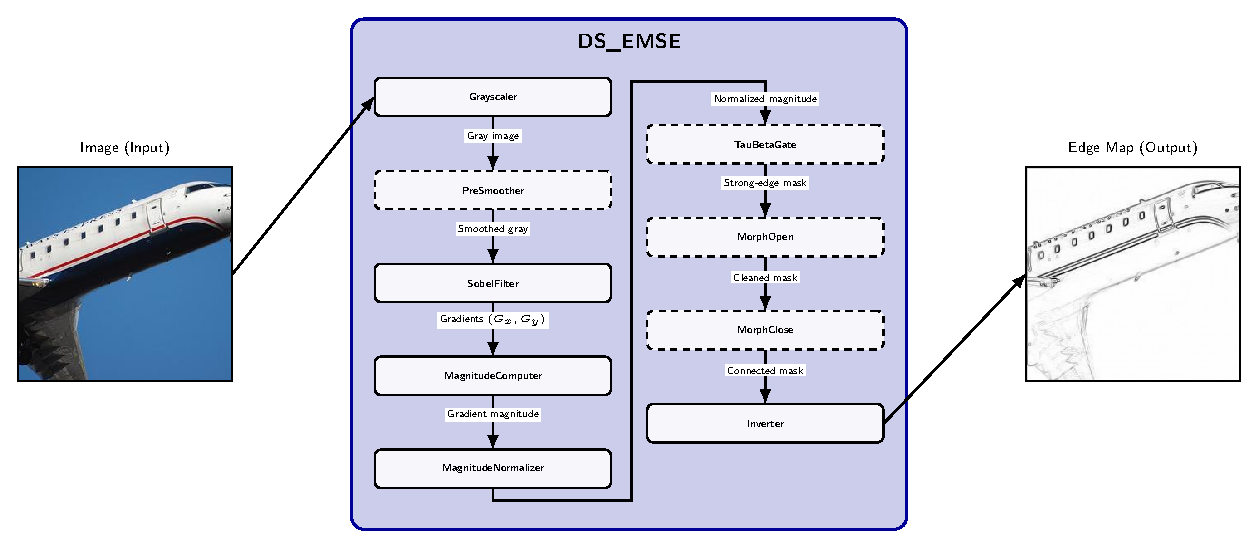
\includegraphics[clip, trim=0cm 0cm 0cm 0cm, width=\VarPicWidthD]{Figures/tikz2pdf/ds_emse/ds_emse.pdf}
    \caption{Ablauf und Parameter der \ac{DS-EMSE}-Methode}
    \label{fig:DS_Emse_Ablauf}
\end{figure}

\newpage

Um die bestmögliche Leistung der DS-EMSE-Methode zu gewährleisten, ergänzen wir diese durch ein dediziertes Tool zur Identifizierung optimaler Parameter. Dieses Konfigurationstool hilft beim Prozess der Parameterwahl. Die in Abbildung \ref{fig:DS_Emse_Ablauf} gestrichelt umrandeten Parameter sind diese, die mit Hilfe des Tools einstellbar sind. Dies stellt sicher, dass die Kantenkarten als primäre Forminformationen die bestmögliche Qualität aufweisen, was die Robustheit des gesamten Trainingsprozesses maßgeblich erhöht.




\subsection{Herausforderung 3: Unzureichende Qualität der generierten Bilder}
Die ursprüngliche Netzarchitektur, die auf CIFAR-10~\cite{krizhevsky2009learning} mit $32 \times 32$ Pixeln ausgelegt ist, ist nicht in der Lage, bei einer Bildauflösung von $256 \times 256$ Pixeln qualitativ hochwertige Ergebnisse zu liefern. Durch die geringe Netztiefe und die auf kleine Eingabedaten optimierte Struktur entstehen Artefakte, unscharfe Bildbereiche und ein unzureichendes Detailniveau. Insbesondere bei hochauflösenden Kantenkarten führt dies dazu, dass wichtige Forminformationen nicht präzise abgebildet werden. Somit ist die vorhandene Architektur für die Anforderungen von ImageNet256~\cite{Uriot2023imageNet} ungeeignet. 




\subsection{Lösungsansatz: Entwurf einer passenden Netzarchitektur}
Um die erhöhte Bildauflösung adäquat zu verarbeiten, wird eine angepasste Netzarchitektur entworfen, die speziell für $256 \times 256$ Pixel optimiert ist. Der neue Aufbau orientiert sich am Encoder-Decoder-Prinzip von SegNet~\cite{badrinarayanan2017segnet}, das durch seine Fähigkeit überzeugt, sowohl globale Kontextinformationen als auch feine Strukturen in den rekonstruierten Ausgaben zu bewahren. 

Die Architektur integriert eine erhöhte Netztiefe mit zusätzlichen Convolutional- und Upsampling-Schichten, wodurch das Repräsentationsvermögen des Generators erweitert wird. Die Encoder-Stufen komprimieren das Eingabebild in eine latente Repräsentation, während die Decoder-Stufen die Bilddetails schrittweise wiederherstellen. Auf diese Weise lassen sich Kanten- und Forminformationen effizient mit hochauflösenden Bilddetails kombinieren. 





\section{Abgrenzung zum Stand der Technik}
\label{sec:AbgrenzungZumStandDerTechnik}
Die Analyse des Originalansatzes von \textcite{He_2023_ICCV} und unsere anfängliche Umsetzung haben gezeigt, dass eine direkte Skalierung auf hochauflösende Bilder erhebliche Herausforderungen mit sich bringt. Das ursprüngliche Konzept ist in seiner Anwendung auf CIFAR-10~\cite{krizhevsky2009learning} limitiert. Die Hauptprobleme liegen in der ineffektiven Nutzung der Kantenkarte durch den Generator, in der Inkompatibilität des ursprünglichen Kantenextraktionsverfahrens für eine effiziente PyTorch-basierte Trainingspipeline sowie in der Netztiefe des Generator-Netzes bei der verwendung von $256 \times 256$ Pixel großen Bildern.

Unsere Arbeit grenzt sich vom Stand der Technik ab, indem wir diese Herausforderungen mit innovativen Lösungsansätzen begegnen. Wir entwickeln eine erweiterte Methode zur dynamischen Texturreduktion, um den Texture-Bias des Generators gezielt zu unterdrücken. Darüber hinaus implementieren wir mit der \ac{DS-EMSE}-Methode ein vollständig differenzierbares und \ac{GPU}-basiertes Kantenextraktionsverfahren, das eine nahtlose Integration in die End-to-End-Trainingspipeline ermöglicht. Zudem entwerfen wir eine Netzarchitektur, die auf einer Bildgröße von $256 \times 256$ Pixel basiert. Dazu greifen wir auf Veröffentlichungen zurück, in denen bereits Encode-Decoder-Netze zur Generierung von Bilddaten behandelt wurden~\cite{badrinarayanan2017segnet, ronneberger2015unet, krizhevsky2009learning, isola2018Pix2Pix}.

Diese methodischen Weiterentwicklungen bilden den Kern unseres endgültigen Konzepts. Ihre detaillierte Beschreibung, einschließlich der genauen architektonischen Spezifikationen und der Implementierung, erfolgt im folgenden Kapitel~\nameref{ch:KonzeptArchitekturImplementierung}.

